\chapter{Úvod do problematiky}
V tejto kapitole si vysvetlíme základne pojmy z biológie a bioinformatiky potrebné pre túto bakalársku prácu,
a popíšeme podobné už existujúce programy.
\section{DNA, gén a genóm}
Deoxyribonukleová kyselina (DNA) je nositeľom genetickej informácie bunky.
Má štruktúru dvojzávitnice, skladajúcej sa z dvoch komplementárnych vlákien.
Vlákno je tvorené nukleotidmi, ktoré obsahujú jednu zo štyroch báz adenín, guanín, tymín a cytozín.
DNA zvykneme zapisovať ako postupnosť týchto báz, kde každú bázu kódujeme jej počiatočným písmenom A,G,T,C.
Vzdialenosť dvoch DNA sekvencií vyjadruje, ako veľmi sú rozdielne.


Gén je súvislý úsek DNA, ktorý kóduje tvorbu proteínu. Gén je základnou jednotkou dedičnosti.


Genóm je súbor DNA molekúl v bunke. Jednotlivé molekuly DNA sa väčšinou nachádzajú v štruktúrach nazývaných chromozómy.
Napríklad v ľudskej bunke je 46 chromozómov, každý obsahujúci jednu molekulu dna \cite{Zve08}.

\section{Evolučná história}\label{sec:evhist}
Evolučná história je postupnosť udalostí, ktoré sa odohrali na nejakej DNA sekvencii.
V tejto práci budem uvažovať iba udalosti ktoré menia poradie alebo počet génov na chromozóme.
Okrem nich sa ale počas evolúcie môžu vyskytnúť aj udalosti, ktoré menia bázy DNA sekvencie,
takéto udalosti môžu ovplyvniť funkciu génu, pre našu prácu však nie sú podstatné
\newline
Budeme uvažovať hlavne tieto udalosti:
\newline
\begin{itemize}
\item \emph{Duplikácia} - skopírovanie génu alebo skupiny génov na iné miesto v DNA.
\item \emph{Inzercia} - vloženie jedného alebo viacerých nových génov.
\item \emph{Delécia} - odstránenie jedného alebo viacerých génov.
\item \emph{Inverzia} - zmena poradia a orientácie génu alebo génov.
\item \emph{Transpozícia} - zmena poradia génu alebo génov.
\item \emph{Speciácia} - špeciálna udalosť, ktorá označuje vznik nového druhu. Vzniká nová vetva v evolučnej histórii.
\end{itemize}

V našej reprezentácii je evolučná história postupnosť krokov, pričom každý krok pozostáva zo známej sekvencie génov na jednom chromozóme určitého organizmu.
Medzi jednotlivými krokmi došlo k jednej alebo viacerým udalostiam. 

\section{Fylogenetický strom}

\begin{figure}[h]
 \centering
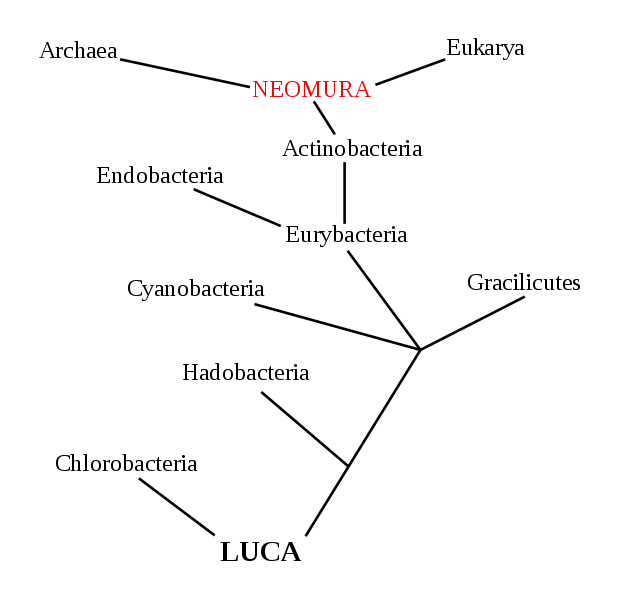
\includegraphics[width=0.6\textwidth]{images/rooted}
\caption{Príklad zakoreneného fylogenetického stromu, Zdroj:  wikipedia.org}\label{obr:rooted}
\end{figure}

Fylogenetický strom reprezentuje evolučné vzťahy medzi sadou objektov. Pokiaľ si za objekty zvolíme biologické druhy, jedná sa o takzvaný \emph{druhový strom}.
Jednotlivé druhy sú pospájané hranami, ktoré reprezentujú evolučný vzťah.
Druhy, ktoré sa nachádzajú na \emph{listoch} stromu, sú buď existujúce druhy, z ktorých sa nevyvinuli nové druhy, alebo vyhynuté druhy bez potomkov.  
Vnútorné vrcholy predstavujú predchodcov, o ktorých sa predpokladá, že sa vyskytli počas evolúcie. 
Každý vnútorný vrchol zodpovedá speciácii, kde z jedného druhu vznikajú dva nové druhy.
Pokiaľ je v strome známy posledný spoločný predok všetkých listov, nazveme ho \emph{koreň}, a takýto strom označíme ako \emph{zakorenený}.
V \emph{zakorenenom} strome je zrejmá orientácia vnútorných hrán, ktorá určuje, ktorý druh sa vyvinul z ktorého.
Na obrázku \ref{obr:rooted} vidíme príklad zakoreneného fylogenetického stromu. Prvok \emph{LUCA} predstavuje posledného univerzálneho spoločného predchodcu.
Na tomto strome vidíme že Eukaryoty a Archeóny sú od seba fylogeneticky menej vzdialené, ako od Baktérií \cite{wiki:phylo}.


\section{Vizualizácia evolučných histórií}
Vizualizácia je spôsob prevodu dát do grafickej formy, ktorú vieme spracovať naším zrakom, najdominantnejším zmyslom, aký máme.
To nám umožňuje okrem lepšieho pochopenia problému aj rýchlu analýzu a odhalenie existujúcich súvislostí a vzorov ktoré sa nachádzajú vo výsledku.

V oblasti  vizualizácie evolučných histórií je najčastejšie zobrazovanie fylogenetických stromov.
Na tento účel existuje množstvo programov  ako napríklad \emph{phylo.io}, \emph{ETE toolkit} alebo \emph{Archaeopteryx} \cite{Robinson_2016,Huerta-Cepas2010,archa}.
Poskytujú vizualizáciu fylogenetických stromov v ktorých gény buď vôbec nevystupujú alebo sa nachádzajú iba pri listoch stromu.
Rozdiely medzi jednotlivými vrcholmi, sa zvyknú zobrazovať vzdialenosťou týchto vrcholov, alebo číslom, ktoré predstavuje vzdialenosť DNA sekvencií týchto vrcholov. 
My však cheme, aby sa vo výslednom zobrazení nachádzali jednotlivé udalosti, ktoré sa odohrali počas evolučnej histórie, podobne ako na obrázku \ref{obr:genetree},
alebo v článku \cite{gorecki2011maximum}. Takéto zobrazenie, v ktorom sa nachádzajú viaceré gény naraz, vidíme na obrázku \ref{obr:tree}, 
zatiaľ však neexistuje používateľsky pohodlný spôsob, ako ho vytvoriť.
Náš program by mal umožniť používateľovi, vytvárať podobné obrázky, s pomocou jednoducho ovládateľnej aplikácie.
\begin{figure}[t]
 \centering
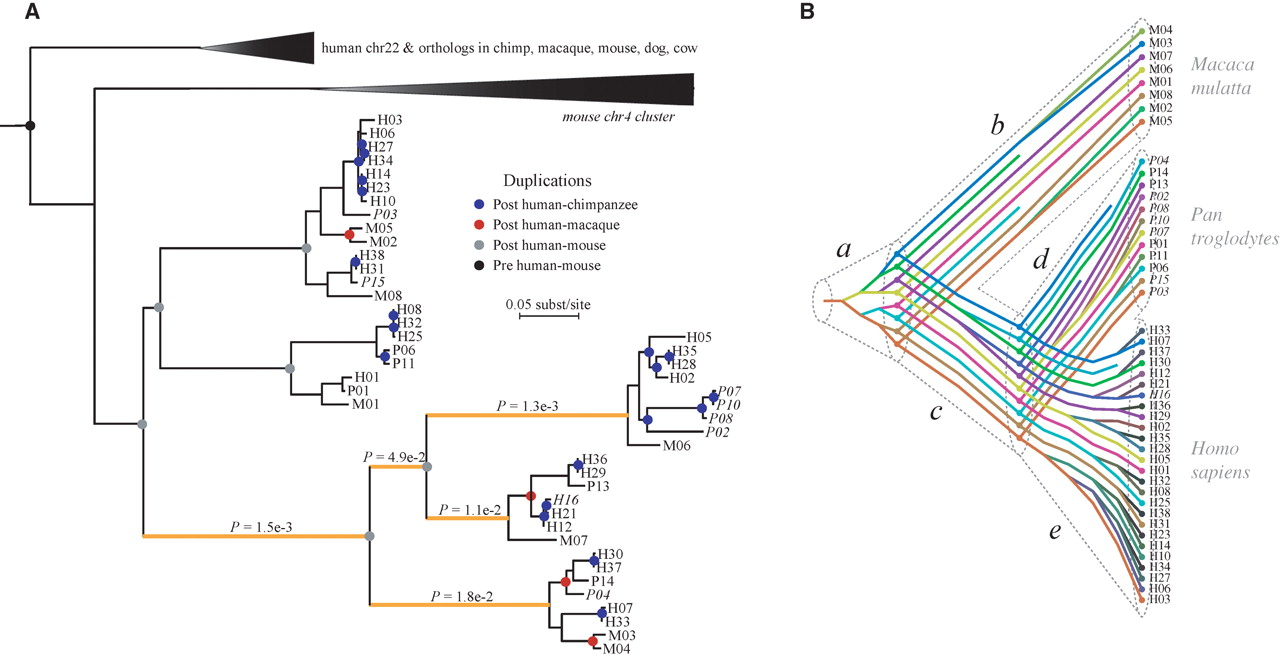
\includegraphics[width=1\textwidth]{images/genetree}
\caption{Zobrazenie evolučnej histórie, v ktorom sledujeme duplikácie pre skupinu génov. V časti \textbf{B} vidíme duplikačnú históriu . Zdroj: \cite{222}}\label{obr:genetree}
\end{figure}

\begin{figure}
\centerline{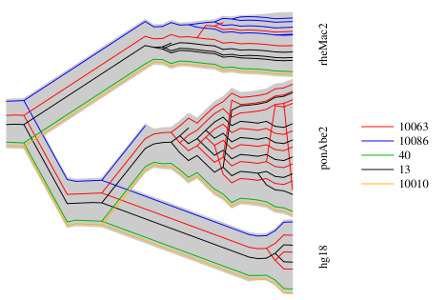
\includegraphics[width=1\textwidth]{images/DUP-tube-tree}}
\caption{Zobrazenie evolučnej histórie viacerých génov naraz,na pozadí sa nachádza druhový strom. Zdroj:\cite{Vinar2010}}\label{obr:tree}
\end{figure}
